%# -*- coding: utf-8-unix -*-
% !TEX program = xelatex
% !TEX root = ../thesis.tex
% !TEX encoding = UTF-8 Unicode
%%==================================================
%% chapter02.tex for SJTU Master Thesis
%% based on CASthesis
%% modified by wei.jianwen@gmail.com
%% Encoding: UTF-8
%%==================================================

\chapter{基于多任务学习的NL2SQL生成}
\label{chap:cnl2sql}
在第\ref{chap:enl2sql}章中,本文结合了深度学习与深度强化学习来解决NL2SQL的问题。
然而,目前所有研究都只是将英文的自然语言问题转换为机器可执行的SQL查询语句,而没有涉及到其他语种的自然语言。
% 如何将中文自然语言问题转换为SQL查询语句?如何进一步提升英文自然语言生成SQL查询语句的准确性?
本章研究提出了基于多任务学习的自然语言生成 SQL 查询语句(NL2SQL)的方法,提升NL2SQL任务中英文自然语言生成SQL查询语句的准确性,以及同时解决中文自然语言问题转换为SQL查询语句的问题。


\section{相关技术}
\subsection{注意力转换器模型}

2017年谷歌提出了注意力转换器模型(Transformer)\cite{vaswani2017attention},其在翻译任务上的表现十分优异。
在该模型中,最重要的机制为多头自注意力机制(multi-head self-attention)和位置编码机制(Positional Encoding)。

\textbf{(1) 多头自注意力机制(multi-head self-attention)}

\begin{figure}[!htp]
  \centering
  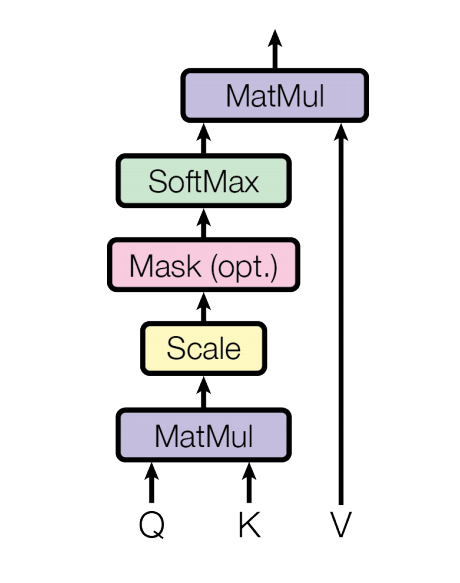
\includegraphics[width=7cm]{example/SDPA.png}
  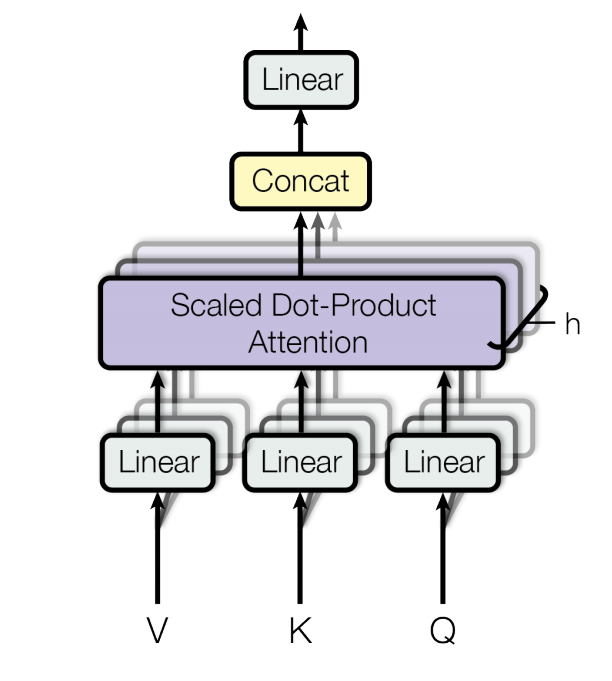
\includegraphics[width=7cm]{example/MHA.png}
  \bicaption[缩放点积注意力和多头注意力]
    {缩放点积注意力(scaled dot-product attention)和多头注意力(multi-head attention)}
    {Scaled Dot-product Attention And Multi-head Attention}
  \label{fig:SDPAMHA}
\end{figure}

多头自注意力机制包含缩放点积注意力(scaled dot-product attention)和多头注意力多头注意力(multi-head attention)两部分,如图\ref{fig:SDPAMHA}所示)。
在缩放点积注意力中,输入由query(Q),$d_k$维的key(K)以及$d_v$维的value(V)组成,需要将query和一些列的(key,value)对映射起来,如公式\ref{cnl2sqleq:mhsaeq1}。
实际上,注意力机制就是一个由诸多Query和(key,value)组成的映射函数。

\begin{equation}
  \label{cnl2sqleq:mhsaeq1}
  q -> [(k_1,v_1),(k_2,v_2),...] -> attention = w_1 * v_1 + w_2 +v_2 + ... 
\end{equation}

query和所有key计算点积,然后除以$\sqrt{d_k}$并计算$softmax$值,得到value对应的权重$w$,如公式\ref{cnl2sqleq:mhsaeq2}。

\begin{equation}
  \label{cnl2sqleq:mhsaeq2}
  Attention(Q,K,V) = softmax(\frac{QK^T}{\sqrt{d_k}})V  
\end{equation}

而多头注意力实际上就是将query和key做多次的线性映射,最后将结果串联在一起。
在编码器和解码器结构中,query来自于上一层的解码器中,而key和value来自上一层的编码器中。
多头注意力就是将句子中的每一个部分都参与到编码和解码的过程中,允许模型关注来自不同位置及不同表示的信息,如公式\ref{cnl2sqleq:mhsaeq3}。

\begin{equation}
  \label{cnl2sqleq:mhsaeq3}
  MultiHead(Q,K,V) = Concat(head_1,...,head_h) \quad \mbox{其中} head_i = Attention(QW^Q_i,KW^K_i,VW^V_i)
\end{equation}

\textbf{(2) 位置编码机制(Positional Encoding)}

鉴于注意力转换器模型并没有CNN或RNN的结构,为了引入序列的位置信息,还需要加入位置编码机制。
在编码器和解码器的嵌入之后的向量与$d_{model}$维的位置编码进行求和。
位置编码的方式有很多种,可以是学习得到的也可以是固定的,可以对不同序列使用$sin$和$cos$函数进行计算,如公式\ref{cnl2sqleq:mhsaeq4}。

\begin{gather}
  \label{cnl2sqleq:mhsaeq4}
  PE_{(pos,2i)} = sin(\frac{pos}{10000^{\frac{2i}{d_{model}}}})\\
  PE_{(pos,2i+1)} = cos(\frac{pos}{10000^{\frac{2i}{d_{model}}}}) 
\end{gather}

\subsection{NLP领域的迁移学习}

在自然语言处理(NLP)领域中有很多重要成果都与迁移学习有关。
例如Word2Vec\cite{mikolov2013efficient},skip-thought Vec\cite{kiros2015skip}和Glove\cite{pennington2014glove}都是先产生预训练好的词向量,再把这些知识“迁移”到其他应用上。
嵌入(embedding)\cite{collobert2008unified,collobert2011natural}、中间表示(intermediate representation)\cite{peters2018deep}和语言模型中的权重\cite{ramachandran2017unsupervised}都可以被迁移到其他类似的架构甚至分类任务\cite{howard2018fine}上。
从机器翻译模型上得到的中间表示可以迁移并提升处理问答、情感分析等任务的模型\cite{mccann2017learned}。
使用问答数据集训练的模型与使用推理数据集训练的模型可以完成对方的任务\cite{min2017question}。
高质量机器翻译模型与低质量机器翻译模型之间也相互支持\cite{zoph2016transfer}。
这些研究表明,想要同时学习中文自然语言查询转换英文自然语言查询和英文自然语言查询生成SQL查询语句两个任务是可以迁移的。

\subsection{NLP领域的多任务学习}

2011年,Collobert\cite{collobert2011natural}首先提出了可以同时处理多个自然语言问题的解决方案,处理的问题包括分块(chunk)、命名实体识别(NER)、词性标注(POS)、语义角色标注(SRE)等。
之后Hashimoto\cite{hashimoto2017joint}也提出了可以同时处理依赖解析、语义相关和自然语言推理任务的网络结构。
使用跨语种的预料进行机器翻译模型训练时发现,采用多任务学习的方法\cite{johnson2017google}甚至可以一定程度解决零样本的问题。
基于序列到序列的模型采用不同数量的编码器和解码器时\cite{luong2015multi}甚至可以同时学习翻译、解析和图像字幕生成的任务。
甚至学习图像分类和语音识别任务的模型可以被模块化\cite{kaiser2017one}之后拓展到图像到文字的问答任务上\cite{xiong2016dynamic}。
采用\cite{ruder2017learning}的方法还可以减轻任务之间存在的干扰。

事实上,早在1997年Caruana\cite{caruana1997multitask}就证明多任务学习是有效的,因为模型能够利用任务之间的关联性。
当同时学习的任务十分相关时,学习不同的任务可以提供归纳偏差\cite{mitchell1980need},强迫模型去学习那些更通用和普遍的表示方法。
通过将许多单独的任务同时学习并比较,可以充分验证多任务学习的有效性\cite{wang2018glue,poliak2018evaluation,poliak2018towards}。

% \subsection{NLP领域的元学习}


\section{解决方案}

本文采用TCR(Task-Content-Result)模板将多任务进行统一,并设计了一种基于多任务学习的神经网络结构实现多项任务的同时学习。

\subsection{TCR模板}

本文中,中文自然语言问题生成SQL查询语句被划分为两个子任务:中文自然语言翻译为英文自然语言任务和英文自然语言问题生成SQL查询语句任务。
在第\ref{chap:enl2sql}章中,本文所提出的基于深度强化学习的解决方案已经可以有效地解决NL2SQL问题,并且在WikiSQL数据集和Spider数据集上有优异的表现。
所以,本文产生了一个非常自然的想法:直接使用翻译工具或翻译软件将中文的自然语言问题直接转换为英文自然语言问题,之后再使用\ref{enl2sql:zqjxqmx}节中提出的增强解析器模型将英文自然语言转换为SQL查询语句。
但是,这种方法会遇到许多问题,如图\ref{fig:cnl2sqlproblem}所示,示例中,中文自然语言均使用谷歌翻译自动翻译为英文自然语言。

\begin{figure}[!htp]
    \centering
    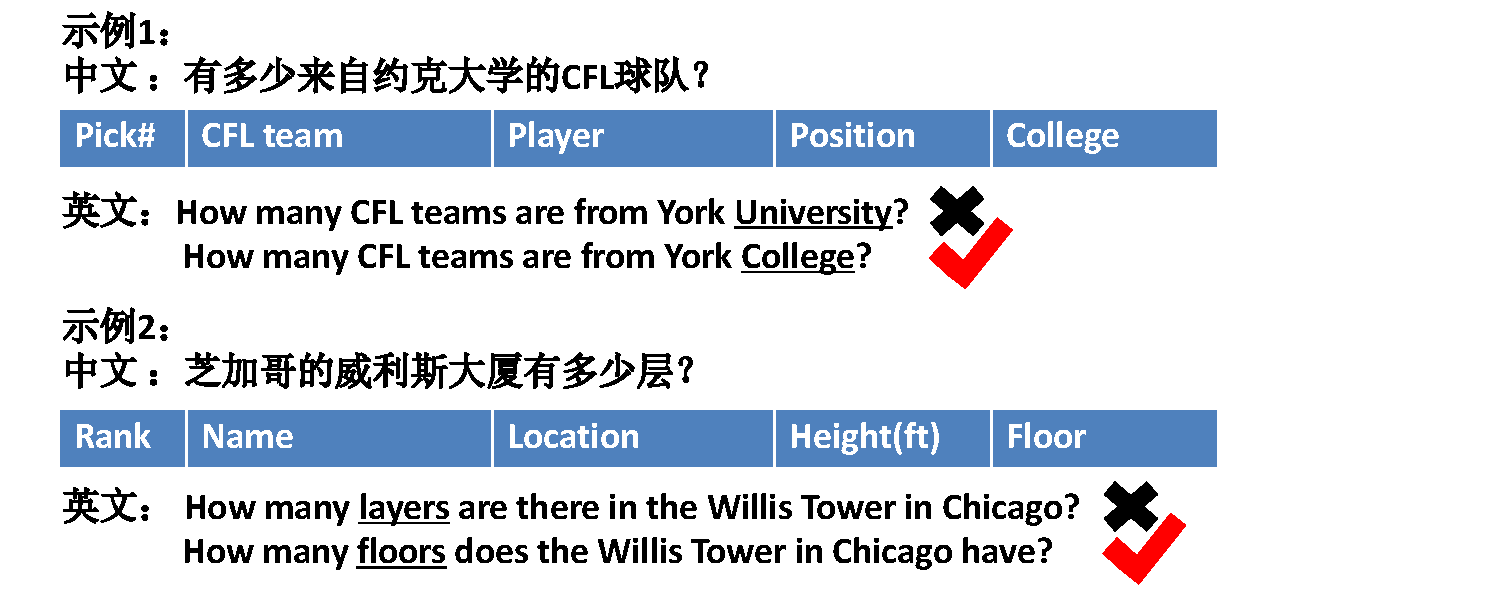
\includegraphics[width=15cm]{example/cnl2sqlproblem.pdf}
    \bicaption[中文自然语言问题生成SQL查询语句的错误示例]
      {中文自然语言问题生成SQL查询语句的错误示例}
      {An Error Example of Chinese Nature Language To SQL Statement}
    \label{fig:cnl2sqlproblem}
  \end{figure}

从图\ref{fig:cnl2sqlproblem}中的示例一可以看出,数据库表模式中的列名为“College”,而谷歌翻译将中文“大学”翻译为“University”。
而示例二中的“层”翻译为了“layers”而不是“floors”。
形如这一类的问题会给SQL的生成带来很大的问题。

究其原因,从中文自然语言到英文自然语言再到SQL查询语句这一过程是一个紧密关联的过程,如果将其拆分为两个部分,则翻译的过程中将会丢失大量的数据库、SQL语言本身的很多信息。
所以,本文提出TCR模板用以将这两个独立的任务有机的统一起来,作为多任务学习网络的输入。

\begin{figure}[!htp]
    \centering
    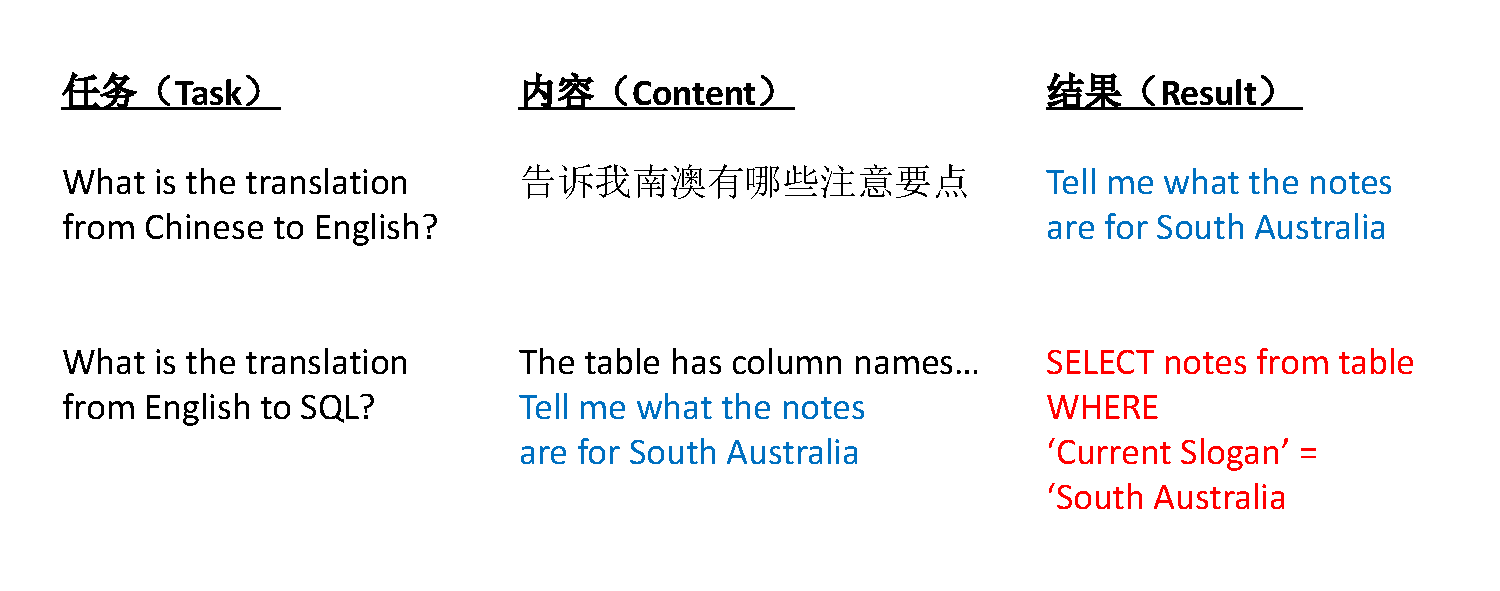
\includegraphics[width=15cm]{example/tcr.pdf}
    \bicaption[TCR模板]
      {TCR模板(任务-内容-结果模板)}
      {TCR Template}
    \label{fig:cnl2sqltcr}
  \end{figure}
%DONE 上图中的任务不要用问句,直接用祈使句。
如图\ref{fig:cnl2sqltcr}所示,本文将中文自然语言翻译为英文自然语言任务和英文自然语言生成SQL查询语句任务使用TCR模板(任务-内容-结果)进行统一。
例如,“告诉我南澳有哪些注意要点”先翻译为英文,其任务为“Please translate Chinese into English.”,
%DONE 任务不要用问句,直接用祈使句。
内容为“告诉我南澳有哪些注意要点”(表明所需要翻译的中文语句),结果为“Tell me what the notes are for South Australia”。
而后再将“Tell me what the notes are for South Australia”转换为SQL查询语句,其任务为“Please translate English into SQL statement.”,
%DONE 任务不要用问句,直接用祈使句。
内容为“The table has column names… Tell me what the notes are for South Australia”(表明数据库模式和英文查询语句),结果为“SELECT notes from table WHERE ‘Current Slogan’ =‘South Australia”,从而完成生成的全过程。

TCR模板将两个任务的模式进行了统一,使得网络模型的输入和输出得以一致,而不用设计两个不同的网络结构来处理这两个任务。
在后文中,本文还将这个模板用于自然语言处理领域中的多项任务中,详见\ref{cnl2sql:syyfx}节。

\subsection{多任务学习网络}

本文使用TCR模板对每个任务进行统一并且在训练阶段采用联合训练的方法,其所使用的神经网络的结构称为多任务学习网络,如图\ref{fig:cnl2sqlnet}所示。
近几年来,有不少研究者所研究的问答模型\cite{wang2016machine,seo2016bidirectional,xiong2017dcn+}的和本文提出的模型较为类似,
%DONE 这些研究者的问答模型要有参考文献引用
他们的问答模型往往假设模型得到的答案片段可以直接从上下文信息中复制,但是本文提出的多任务学习网络适用于更复杂的问答场景。
%done 为何是问答?是否是指端到端模型、端到端转换?(不完全是,有很多人把机器阅读理解(问题,文章段落,答案)的模型和其他类似的模型统称为问答模型(Question Answering),本文的多任务学习网络模型类似于问答模型,不过更加泛化)
在之前的TCR模板中,任务对应于问答模型中的问题,内容对应于问答模型中的上下文,而结果对应于问答模型中的回答。
由于TCR模板中的任务往往包含限制搜索空间的非常关键的信息,本文会在多任务学习网络中使用了协同注意力机制\cite{vaswani2017attention}并加以拓展,从而使得对模型输入的表示更加丰富。
此外,多任务学习网络还采用了指针机制\cite{vinyals2015pointer},并将其改造为分层的多指针生成器,使得网络能够直接从任务和内容中进行文本的复制。

\begin{figure}[!htp]
  \centering
  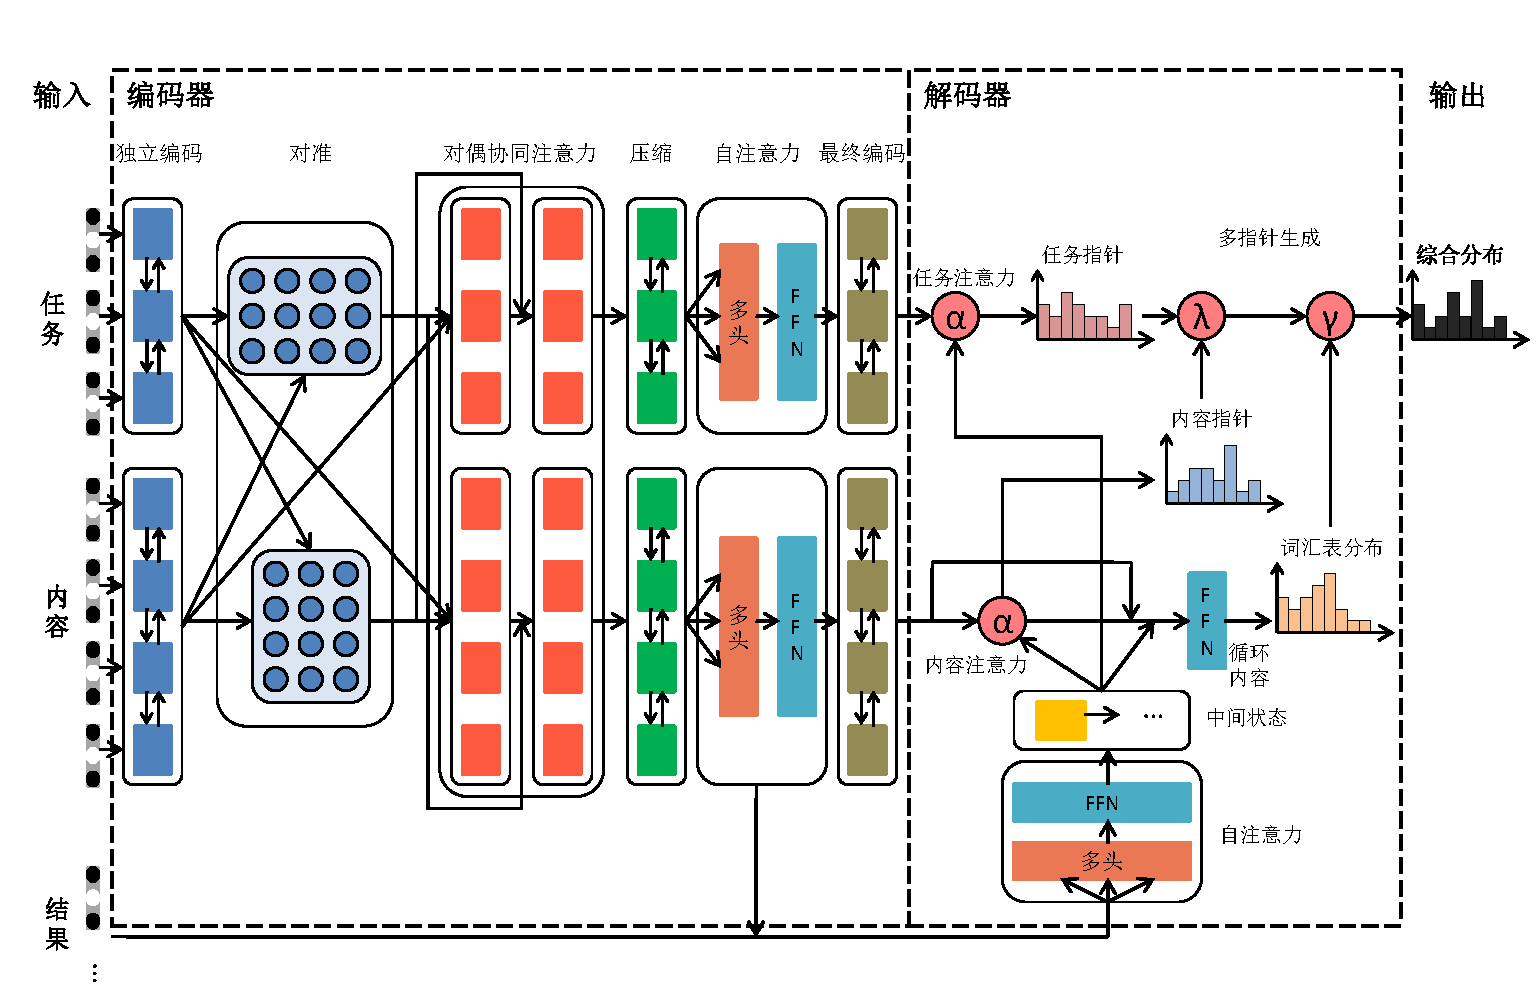
\includegraphics[width=15cm]{example/cnl2sqlnet.pdf}
  \bicaption[多任务学习网络结构]
    {多任务学习网络结构}
    {The Architecture of Multitasking Learning Network}
  \label{fig:cnl2sqlnet}
\end{figure}
%done上图中只有一个任务,上次和你讲过,要再画一个图,把多个任务画出来,并表达出多任务学习时的迁移学习的思路,要有编码器和解码器。

在训练阶段,多任务学习网络的输入序列由三个部分组成,分别为:由$l$个单词构成的内容$c$;
由$m$个单词构成的任务$q$;由$n$个单词构成的结果$a$。
其中,每个输入序列都是一个矩阵,矩阵中的第$i$行对应于序列中的第$i$个词的嵌入(embedding)(可为字符向量或词向量),维度为$d_{emb}$。有公式\ref{cnl2sqleq:drwwl1}:
\begin{equation}
    \label{cnl2sqleq:drwwl1}
    C \in \mathbb{R}^{l \times d_{emb}} \qquad Q \in \mathbb{R}^{m \times d_{emb}} \qquad A \in \mathbb{R}^{n \times d_{emb}}
  \end{equation}

此外,多任务网络的不同任务之间的迁移过程如图\ref{fig:cnl2sqltransfer}所示,
图中黑色方框中的内容为多任务网络的简化图。
可以看到,任务一训练完成时的对偶协同注意力中的参数可以被直接作为任务二对应参数的初始状态,这一过程也叫做微调(Fine tuning)。
网络在其他任务上所学习到的一些表示可以通过这种方式进行迁移。
在实验阶段,本文在多任务学习中还使用了不同的训练策略进行优化,详见\ref{cnl2sql:btyhclxdsyjg}。
  \begin{figure}[!htp]
    \centering
    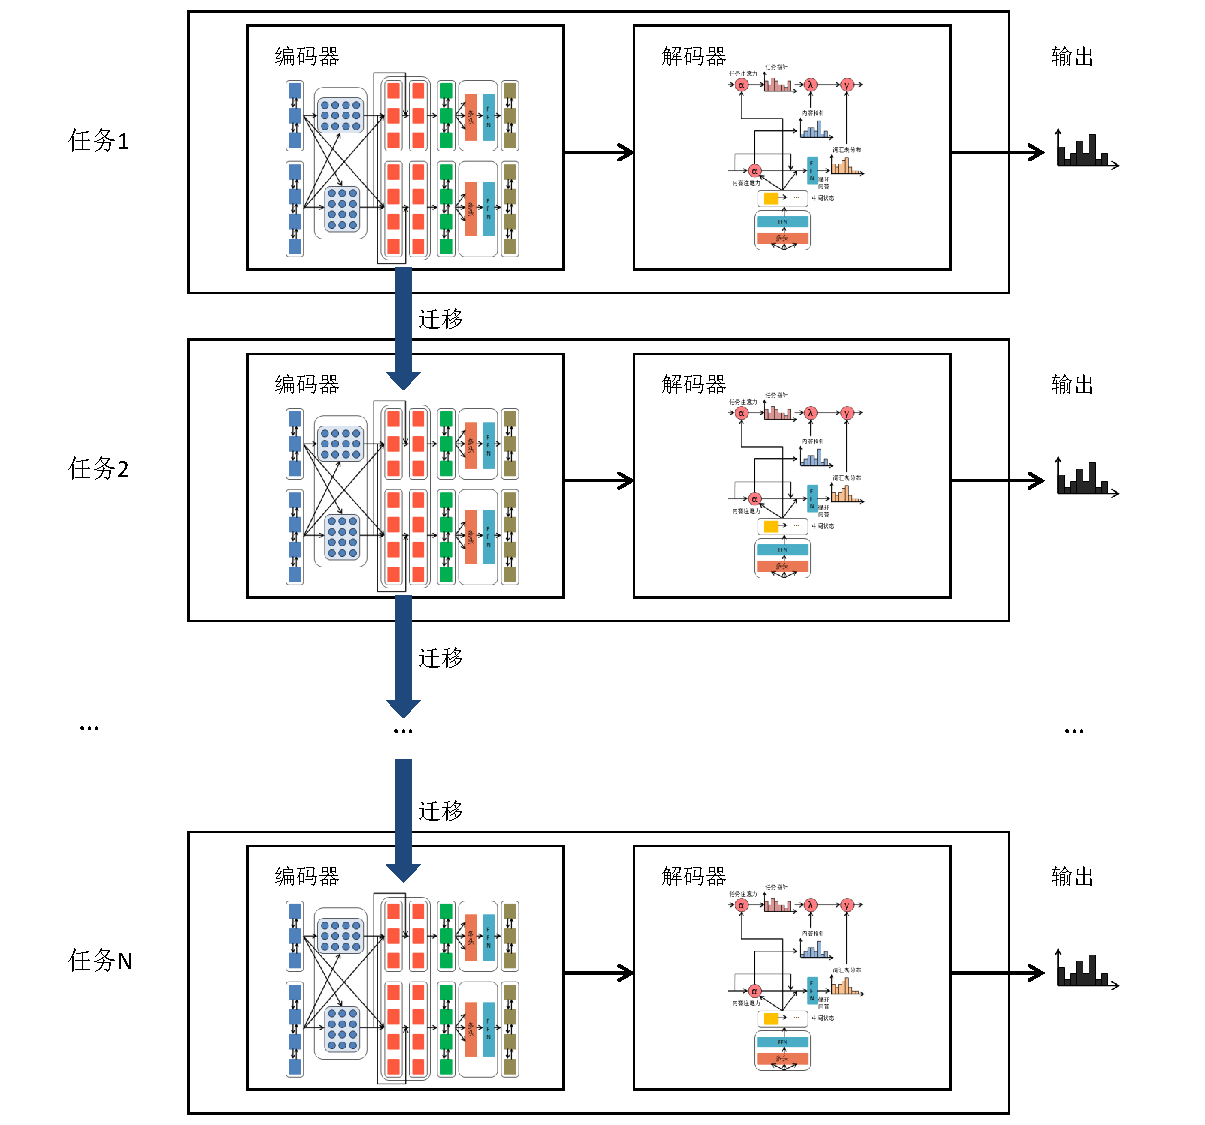
\includegraphics[width=15cm]{example/cnl2sqltransfer.pdf}
    \bicaption[任务间的迁移学习]
      {任务间的迁移学习}
      {Transfer Learning Between Tasks}
    \label{fig:cnl2sqltransfer}
  \end{figure}

接下来,本文将分别详细阐述多任务学习网络中的编码器和解码器。

\subsection{编码器}
\label{cnl2sql:encoder}

编码器将内容矩阵$C$、任务矩阵$Q$和结果矩阵$A$作为输入,
使用深度栈式循环神经网络,结合协同注意力机制(coattention)和自注意力机制(self-attention),
来生成编码阶段的最终的表示$C_{fin} \in \mathbb{R}^{l \times d}$和$Q_{fin} \in \mathbb{R}^{m \times d}$(即编码之后的内容信息和任务信息),
并且还可以让网络学习到他们之间的局部和全局的相互依赖关系。
编码器的工作流程由六个阶段组成:

\textbf{(1) 独立编码阶段}
%done 小标题要有编号,余同修改

首先使用一个简单的线性层将输入矩阵投射到$d$维的空间上,如公式\ref{cnl2sqleq:encoder1}。
\begin{equation}
    \label{cnl2sqleq:encoder1}
    CW_1 = C_{proj} \in \mathbb{R}^{l \times d} \qquad QW_1 = Q_{proj} \in \mathbb{R}^{m \times d} 
  \end{equation}
这些投射之后的表示将被输入给一个共享的双向长短期记忆网络(bi-LSTM)\cite{hochreiter1997long,graves2005framewise}[!脚注!],如公式\ref{cnl2sqleq:encoder2}。
\begin{equation}
    \label{cnl2sqleq:encoder2}
    BILSTM_{ind}(C_{proj}) = C_{ind} \in \mathbb{R}^{l \times d} \qquad BILSTM_{ind}(Q_{proj}) = Q_{ind} \in \mathbb{R}^{l \times d}
\end{equation}

\textbf{(2) 对准阶段}

在获得协同注意力的表达之前,需要先对每个序列的编码表达进行对准。
我分别给$C_{ind}$和$Q_{ind}$增加一个预训练的嵌入使得现在的$C_{ind} \in \mathbb{R}^{(l+1) \times d}$以及$Q_{ind} \in \mathbb{R}^{(m+1) \times d}$,
这样做可以让每个单词不会和序列中的某个单词强制对准。

令$softmax(X)$表示逐列进行softmax操作,即矩阵$X$中的每列进行标准化后的和为1。
本文将内容信息的序列表示与任务序列表示之间进行点积计算得到相似性得分,并使用归一化操作来获得数据的对准,如公式\ref{cnl2sqleq:encoder3}:
\begin{equation}
  \label{cnl2sqleq:encoder3}
  softmax(C_{ind}Q_{ind}^{\top}) = S_{cq} \in \mathbb{R}^{(l+1) \times (m+1)} \qquad softmax(Q_{ind}C_{ind}^{\top}) = S_{qc} \in \mathbb{R}^{(m+1) \times (l+1)}
\end{equation}

\textbf{(3) 对偶协同注意力阶段}

再对准之后,要去计算一个序列中的某个单词和另一个序列中相关的单词的加权求和,如公式\ref{cnl2sqleq:encoder4}。
\begin{equation}
  \label{cnl2sqleq:encoder4}
  S_{cq}^{\top}C_{ind} = C_{sum} \in \mathbb{R}^{(m+1) \times d} \qquad S_{qc}^{\top}Q_{ind} = Q_{sum} \in \mathbb{R}^{(l+1) \times d}
\end{equation}

对偶协同注意力就是要通过同样的权重将对准时得到的信息传递给原序列,如公式\ref{cnl2sqleq:encoder5}。
\begin{equation}
  \label{cnl2sqleq:encoder5}
  S_{qc}^{\top}C_{sum} = C_{coa} \in \mathbb{R}^{(l+1) \times d} \qquad S_{cq}^{\top}Q_{sum} = Q_{coa} \in \mathbb{R}^{(m+1) \times d}
\end{equation}

可以发现,进行了加权求和和协同注意力的表示中的第一列为之前添加进去的冗余的嵌入。
在这里不再需要这一个嵌入,所以将矩阵中的这一列去除掉,得到$C_{coa} \in \mathbb{R}^{l \times d}$和$Q_{coa} \in \mathbb{R}^{m \times d}$。

\textbf{(4) 压缩阶段}

为了将对偶协同注意力操作之前的信息压缩至$d$维,接着把之前得到的四种序列表示进行拼接并输入一个单独的双向LSTM中,如公式\ref{cnl2sqleq:encoder6}。
\begin{align}
  \label{cnl2sqleq:encoder6}
  BiLSTM_{comC}([C_{proj};C_{ind};Q_{sum};C_{coa}]) =  C_{com} \in \mathbb{R}^{m \times d}\\
  BiLSTM_{comQ}([Q_{proj};Q_{ind};C_{sum};Q_{coa}]) =  Q_{com} \in \mathbb{R}^{m \times d}
\end{align}

\textbf{(5) 自注意力阶段}

接着,使用一个多头的放缩点积注意力机制(multi-head, scaled dot-product attention)\cite{vaswani2017attention}来捕获每个序列内部的长距离的依赖性,其表达式为公式\ref{cnl2sqleq:encoder7}。

\begin{gather}
  \label{cnl2sqleq:encoder7}
  Attention(\widetilde{X},\widetilde{Y},\widetilde{Z}) = softmax\{\frac{\widetilde{X}\widetilde{Y}^{\top}}{\sqrt{d}}\} \widetilde{Z}\\
  MultiHead(\widetilde{X},\widetilde{Y},\widetilde{Z}) = [h_1;\cdots;h_p]W^o \qquad \mbox{其中}h_j= Attention(\widetilde{X}W^{\widetilde{X}}_j,\widetilde{Y}W^{\widetilde{Y}}_j,\widetilde{Z}W^{\widetilde{Z}}_j)
\end{gather}

公式\ref{cnl2sqleq:encoder7}中变换都为线性变换,所以多头注意力机制可以维持$d$维不变,有公式\ref{cnl2sqleq:encoder8}:
\begin{equation}
  \label{cnl2sqleq:encoder8}
  MultiHead_C(C_{com},C_{com},C_{com}) = C_{mha} \qquad MultiHead_Q(Q_{com},Q_{com},Q_{com}) = Q_{mha}
 \end{equation}

之后,本文使用了一个残差前馈网络(feedforward networks,简称FFN)如公式\ref{cnl2sqleq:encoder9},其中$U \in \mathbb{R}^{d \times f}$,$V \in \mathbb{R}^{f \times d}$。其激活函数为Relu函数\cite{Nair2010Rectified,vaswani2017attention},并且在输入和输出都使用了正则化(layer normalization)\cite{Ba2016Layer}。
\begin{gather}
  \label{cnl2sqleq:encoder9}
  FFN(X) = \max(0,XU)V + X\\
  FFN_C(C_{com} + C_{mha}) = C_{self} \in \mathbb{R}^{l \times d} \qquad FFN_Q(Q_{com} + Q_{mha}) = Q_{self} \in \mathbb{R}^{m \times d}
\end{gather}

\textbf{(6) 最终编码阶段}

最后,使用两个双向LSTM将所有信息进行汇总并将矩阵$C_{fin}$和$Q_{fin}$输入给解码器,如公式\ref{cnl2sqleq:encoder10}。
\begin{equation}
  \label{cnl2sqleq:encoder10}
  BiLSTM_{finC}(C_{self}) = C_{fin} \in \mathbb{R}^{l \times d} \qquad BiLSTM_{finQ}(Q_{self}) = Q_{fin} \in \mathbb{R}^{m \times d} 
\end{equation}


\subsection{解码器}
\label{cnl2sql:decoder}

在编码器得到最终的表示$C_{fin} \in \mathbb{R}^{l \times d}$和$Q_{fin} \in \mathbb{R}^{m \times d}$(即编码之后的内容信息和任务信息)后进入到解码器解码。
解码器的工作流程由六个阶段组成:

\textbf{(1) 结果表示阶段}
%DONE 小标题要有编号,余同修改

在训练阶段,解码器首先要将结果$a$的表示投射到$d$维的空间上,如公式\ref{cnl2sqleq:decoder1}

\begin{equation}
  \label{cnl2sqleq:decoder1}
  AW_2 = A_{proj} \in \mathbb{R}^{n \times d} 
\end{equation}

之后紧接的是一个自注意力层,该注意力层与编码器中的自注意力层相对应。
由于该过程不包含循环和卷积操作,所以为$A_{proj}$加上了一个位置编码信息$x$,如公式\ref{cnl2sqleq:decoder2}。
\begin{equation}
  \label{cnl2sqleq:decoder2}
  A_{proj} + PE = A_{ppr} \in \mathbb{R}^{n \times d},\qquad \mbox{其中} PE[t,k] = \{   
  \begin{array}{lr}
    sin(\frac{t}{10000^{\frac{k}{2d}}}) &  k\mbox{为偶数}\\
    cos(\frac{t}{10000^{\frac{k-1}{2d}}}) &  k\mbox{为奇数}
  \end{array}
\end{equation}

\textbf{(2) 自注意力阶段}

接着使用自注意力机制\cite{vaswani2017attention}从而使得解码器能够知道之前的输出(若之前没有输出则认为之前的输出为某个初始化的单词)和相关内容是什么,从而产生下一个输出。
在多头的注意力机制之后使用了一个残差前馈网络(FFN,其定义在\ref{cnl2sql:encoder}节中的自注意力阶段给出),如公式\ref{cnl2sqleq:decoder3}。

\begin{gather}
  \label{cnl2sqleq:decoder3}
  MultiHead_A(A_{ppr},A_{ppr},A_{ppr}) = A_{mha} \in \mathbb{R}^{n \times d}\\
  MultiHead_{A}C((A_{mha} + A_{ppr}),C_{fin},C_{fin}) = A_{ac} \in \mathbb{R}^{n \times d}\\
  FFN_A(A_{ac} + A_{mha} + A_{ppr}) = A_{self} \in \mathbb{R}^{n \times d}
\end{gather}

\textbf{(3) 获得中间状态阶段}

之后,使用一个标准的带注意力机制的LSTM网络来对每个时刻$t$产生一个内容状态$\widetilde{c}_t$。
这个LSTM又将使用之前的结果序列中的单词$A^{t-1}_{self}$和内容状态来生成一个中间状态$h_t$,如公式\ref{cnl2sqleq:decoder4}。

\begin{equation}
  \label{cnl2sqleq:decoder4}
  LSTM([(A_{self})_{t-1};\widetilde{c}_{t-1}],h_{t-1})= h_t \in \mathbb{R}^{d} 
\end{equation}

\textbf{(4) 任务与内容注意力阶段}

上一阶段中的中间状态可用来获得注意力权重$\alpha^C_t$以及$\alpha^Q_t$,解码器从而可以获得$t$时刻的编码信息,如公式\ref{cnl2sqleq:decoder5}。

\begin{equation}
  \label{cnl2sqleq:decoder5}
  softmax(C_{fin}(W_2 h_t)) = \alpha^C_t \in \mathbb{R}^{l} \qquad softmax(Q_{fin}(W_3 h_t)) = \alpha^Q_t \in \mathbb{R}^{m}
\end{equation}

\textbf{(5) 获得内容与任务状态阶段}

内容的表示将于这些权重相结合并输入给一个前馈网络从而形成内容状态与任务状态,激活函数为$tanh$,如公式\ref{cnl2sqleq:decoder6}。
\begin{equation}
  \label{cnl2sqleq:decoder6}
  tanh(W_4[C^{\top}_{fin}\alpha^C_t;h_t] = \widetilde{c}_{t} \in \mathbb{R}^{d} \qquad tanh(W_5[Q^{\top}_{fin}\alpha^Q_t;h_t] = \widetilde{q}_{t} \in \mathbb{R}^{d}
\end{equation}

\textbf{(6) 多指针生成阶段}

由于本文的模型必须要能够生成那些未出现在任务或内容序列中的单词,所以需要额外声明一个词汇表$v$。
从任务、内容和外部的词汇表中分别获得每个单词的概率分布,如公式\ref{cnl2sqleq:decoder7}。

\begin{gather}
  \label{cnl2sqleq:decoder7}
  \sum_{i:c_i=w_t} (\alpha^C_t)_i = p_c(w_t) \in \mathbb{R}^{n}\\
  \sum_{i:q_i=w_t} (\alpha^Q_t)_i = p_q(w_t) \in \mathbb{R}^{m}\\
  softmax(W_v\widetilde{c}_t) = p_v(w_t) \in \mathbb{R}^{v}
\end{gather}

这些概率分布将会覆盖任务、内容和外部词汇表中所有单词的集合,其中的一些条目将会被赋为0值从而使所有分布都在$\mathbb{R}^{l+m+v}$。
最后,本文设置两个标量开关来调节每个分布的重要程度并确认最终输出的分布,如公式\ref{cnl2sqleq:decoder8}。
\begin{gather}
  \label{cnl2sqleq:decoder8}
  \sigma (W_{pv}[\widetilde{c}_t;h_t;(A_{self})_{t-1}]) = \gamma \in [0,1]\\
  \sigma (W_{cq}[\widetilde{q}_t;h_t;(A_{self})_{t-1}]) = \lambda \in [0,1]\\
  \gamma p_v(w_t) + (1 - \gamma)[\lambda p_c(w_t) + (1 - \lambda)p_q(w_t)] = p(w_t) \in \mathbb{R}^{l+m+v}
\end{gather}

需要说明的是,在训练的全时域中,本文采用的是单词级别的对数似然损失,如公式\ref{cnl2sqleq:decoder9}。

\begin{equation}
  \label{cnl2sqleq:decoder9}
  \mathcal L = -\sum^T_t \log p(a_t)
\end{equation}


\section{实验与分析}
\label{cnl2sql:syyfx}
\subsection{多任务学习实验}

\begin{table}[!htpb]
  \bicaption[多任务学习网络的实验结果]
    {多任务学习网络的实验结果}
    {The Experiment Result of Multitasking Network}
  \label{tab:drwwldsyjg}
  \centering
  \begin{threeparttable}[b]
     \begin{tabular}{cccccccccc}
      \toprule
      \multirow{2}{18mm}{数据集}&\multicolumn{4}{c}{单任务} & \multicolumn{5}{c}{多任务}\\
      \cmidrule(lr){2-5}\cmidrule(lr){6-10}
      & S2S & w/SAtt & +CAtt & +QPtr & S2S & w/SAtt & +CAtt & +QPtr & +ACurr\\
      \midrule
      % 增强解析器(静态预言) & 87.1 & 88.2 & 65.9 & 67.5\\
      % 增强解析器(非确定性预言, 不解决过滤条件顺序问题) & 88.1 & 89.2 & 68.3 & 69.1\\
      WikiSQL & 60.0 & 72.4 & 72.3 & 72.6 & 45.8 & 64.8 & 72.9 & 74.0 & 78.7\\
      IWSLT & 25.0 & 23.3 & 26.0 & 25.5 & 14.2 & 23.6 & 29.0 & 26.1 & 29.7\\
      SQuAD & 48.2 & 68.2 & 74.6 & 75.5 & 47.5 & 66.8 & 71.8 & 70.8 & 74.3\\
      CNN/DM & 19.0 & 20.0 & 25.1 & 24.0 & 25.7 & 14.0 & 15.7 & 23.9 & 24.6\\
      MNLI & 67.5 & 68.5 & 34.7 & 72.8 & 60.9 & 69.0 & 70.4 & 70.5 & 69.2\\
      SST & 86.4 & 86.8 & 86.2 & 88.1 & 85.9 & 84.7 & 86.5 & 86.2 & 86.4\\
      QA-SRL & 63.5 & 67.8 & 74.8 & 75.2 & 68.7 & 75.1 & 76.1 & 75.8 & 77.6\\
      QA-ZRE & 20.0 & 19.9 & 16.6 & 15.6 & 28.5 & 31.7 & 28.5 & 28.0 & 34.7\\
      WOZ & 85.3 & 86.0 & 86.5 & 84.4 & 84.0 & 82.8 & 75.1 & 80.6 & 84.1\\
      MWSC & 43.9 & 46.3 & 40.4 & 52.4 & 52.4 & 43.9 & 37.8 & 48.8 & 48.4\\
      \midrule
      总得分 & - & - & - & - & 483.6 & 566.4 & 543.8 & 584.7 & 607.7\\
      \bottomrule
    \end{tabular}
  \end{threeparttable}
\end{table}

本次实验中,本文不仅将中英翻译任务(IWSLT)与NL2SQL任务(WikiSQL)进行同时学习,而且还加入了阅读理解(SQuAD)、摘要(CNN/DM)、自然语言推理(MNLI)、情绪识别(SST)、语义角色标注(QA-SRL)、关系抽取(QA-ZRE)、对话系统(WOZ)、语义解析(MWSC)任务进行多任务学习。
需要说明的是,每个任务的评价指标不一致,例如:IWSLT的指标为BLEU,WikiSQL的指标为逻辑形式准确率等等。

实验结果如表\ref{tab:drwwldsyjg}所示,
%done 表号不对,余同修改
表中S2S代表序列到序列(sequence to sequence)模型,(w/SAtt)代表增加带自注意力机制的S2S模型,
(+CAtt)代表将任务与内容序列拆分为两个输入序列并增加对偶协同注意力机制,(+QPtr)代表增加任务指针器, (+ACurr)代表增加反递进学习过程。
总得分表示多任务学习时各个子任务得分的和,由于单任务不存在多任务的得分和所以标记为’-’。
模型的训练样本为包含任务序列、内容序列以及结果序列的三元组。
本文所做的对比实验的基准为使用了指针生成器的序列到序列的模型(简称S2S模型)\cite{See2017Get}。
不一样的是,S2S模型的输入为自然语言问题序列,而多任务学习网络的输入为任务及内容序列的集合。

\textbf{(1) 单任务模式下的实验结果}

从表\ref{tab:drwwldsyjg}中的数据可以看出,在单任务的模式下,S2S模型在WikiSQL数据集上的得分比之前的序列到序列的基准方案要高,而多任务学习网络(+QPtr)的效果更加优异,但S2S模型在SQuAD等任务上的效果较差。
在S2S模型的基础上增加了带自注意力机制层(w/SAtt)的编码器和解码器之后\cite{vaswani2017attention},模型具备了整合来自任务和内容信息的能力。
从表中可以看出,新的模型在SQuAD任务上提升了20 nF1,QA-SRL任务上提升了4 nF1,WikiSQL上提升了12 LFEM。
模型在WikiSQL上的表现接近了最高水平的范围,在没有使用结构化的方法\cite{dong2018coarse,huang2018natural,yu2018typesql}下达到了72.4\%。

接着,本文尝试将任务和内容从输入中进行拆分并增加了对偶协同注意力机制(+CAtt)。
可以看到,模型在SQuAD和QA-SRL上的性能提升了超过5 nF1,但是在其他任务上没有明显的提升,甚至在MNLI和MWSC任务上的性能有所降低。
其原因是由于两个任务往往能够从输入中直接复制一些单词作为输出,S2S模型的输入为任务和内容信息的集合,所以其中的指针生成器可以直接完成从输入中复制信息到输出的操作。
而将任务和内容信息拆分为两个输入序列的时候,模型就失去了这个能力。

为了解决这个问题,本文在之前的模型上又增加了一个任务指针(+QPtr)进行实验。
实验结果显示,任务指针有效的提高了模型在MNLI和MWSC上的性能。
同时,模型在SQuAD任务上提升到了75.5 nF1,达到了SQuAD领域中使用直接跨度检测方法的水平,也就是说多任务学习网络达到了不明确将问题进行跨度检测的方法中的最高水平。

最后的模型在WikiSQL任务上达到了72.6\%的逻辑形式准确率以及80.4\%的数据库执行准确率,超过了之前的最高水平\cite{dong2018coarse}的71.7\%和78.5\%。

\textbf{(2) 多任务模式下的实验结果}

从表\ref{tab:drwwldsyjg}中的数据可以看出,在多任务的模式下,S2S模型在很多任务下的表现相比于单任务模式还要更差,模型的总得分只有473.6分。
而增加了带自注意力机制层(w/SAtt)、对偶协同注意力机制(+CAtt)、任务指针(+QPtr)后模型的表现越来越好,达到了584.7分。
充分说明了模型在多任务场景下具有很好的通用性和可拓展性。
多任务与单任务模型相比,在QA-ZRE任务上的F1得分又有11点提升,也验证了多任务的模型在解决零样本学习(zero-shot learning)上的能力。

更为重要的是,在多任务模式下WikiSQL任务的逻辑形式准确率为74.0\%、数据库执行准确率为83.4\%,使用反递进学习策略下的性能更加优秀,达到78.7\%和86.1\%详见\ref{cnl2sql:btyhclxdsyjg}节。

\subsection{优化策略实验}
\label{cnl2sql:btyhclxdsyjg}

\begin{table}[!htpb]
  \bicaption[多任务学习网络在不同训练策略下的实验结果]
    {多任务学习网络在不同训练策略下的实验结果}
    {The Experimental Results of Multitasking Networks With Different Strategies}
  \label{tab:drwwlzbtxlclxdsyjg}
  \centering
  \begin{threeparttable}[b]
     \begin{tabular}{cccccc}
      \toprule
      \multirow{2}{18mm}{数据集}&\multirow{2}{18mm}{完全联合}&\multirow{2}{18mm}{递进} & \multicolumn{3}{c}{反递进}\\
      \cmidrule(lr){4-6}
      % & S2S & w/SAtt & +CAtt & +QPtr & S2S & w/SAtt & +CAtt & +QPtr & +ACurr\\
      & & & SQuAD & +IWSLT+CNN/DM & +MNLI\\
      \midrule
      WikiSQL & 62.0 & 68.6 & 78.7 & 54.8 & 42.6\\
      IWSLT & 16.1 & 4.3 & 29.7 & 18.7 & 19.0\\
      SQuAD & 70.8 & 43.4 & 74.3 & 74.5 & 74.6\\
      CNN/DM & 23.9 & 21.3 & 24.6 & 20.8 & 21.6\\
      MNLI & 70.5 & 58.9 & 69.2 & 69.6 & 72.7\\
      SST & 86.2 & 84.5 & 86.4 & 83.6 & 86.8\\
      QA-SRL & 75.8 & 70.6 & 77.6 & 77.5 & 75.1\\
      QA-ZRE & 28.0 & 24.6 & 34.7 & 30.1 & 37.7\\
      WOZ & 80.6 & 81.9 & 84.1 & 81.7 & 85.6\\
    
      MWSC & 48.8 & 41.5 & 48.4 & 34.9 & 41.5\\
      \midrule
      % 总得分 & - & - & - & - & 473.6 & 546.4 & 533.8 & 562.7 & 571.7\\
      总得分 & 562.7 & 499.6 & 607.7 & 546.2 & 557.2\\
      \bottomrule
    \end{tabular}
  \end{threeparttable}
\end{table}

在多任务的训练过程中本文还进行了多种批量采样(batch-level sampling)策略的实验,包括联合训练、递进学习、反递进学习等,其实验结果如表\ref{tab:drwwlzbtxlclxdsyjg}所示。

首先考虑的是完全联合(fully joint)的策略。
从训练开始到结束,对所有的任务按照固定的顺序循环的进行批量采样。
这种策略在迭代(iteration)次数较少的单任务下的表现良好,见表\ref{tab:drwwlzbtxlclxdsyjg},但在迭代次数较多的单任务下性能不佳。
经过总结,本文发现单任务与多任务场景下的性能的差异与单任务的迭代次数之间有很强的关联。

由于上述原因,本文还尝试了一些反递进学习的策略\cite{Bengio2009Curriculum}。
这些训练的策略都是由两阶段组成的:1)在第一阶段中对部分任务进行联合训练(往往选择较难的任务)。2)第二阶段根据完全联合策略进行对所有任务进行训练。

首先,尝试先将SQuAD任务进行单独训练,之后再对其他的所有任务进行完全联合训练。
由于多任务学习网络对于所有任务来说是一种基于问答的方法,所以联想到是否可以先与训练SQuAD这样的QA数据集然后再对其他的类QA的任务进行训练。
这种方法可以使得解码器先学会如何从内容信息中检索出有用信息,然后学习不同的任务以及如何产生属于不同任务领域的单词。
在SQuAD这个任务场景下进行预训练已经被证明可以提高NLI的性能\cite{min2017question}。
根据实验结果来看,这种方式相对于其他的训练策略而言是一种更有效的训练策略,在总得分上获得了607.7的最高分。
需要特别提到的是,这种策略在IWSLT任务上的得分较低,但是在其他的任务中会有更大的提升,特别是使用指针的任务。

为了探索在递进学习策略的初始状态下增加额外的任务是否会进一步提高性能,本文还尝试了将IWSLT、CNN/DM任务和IWSLT、CNN/DM、MNLI任务加入到第一阶段进行训练。
这些任务包含了与其他任务非常相关的训练样本,并且也包含了最长的结果序列。
除此之外,这些任务具有很高的多样性,应该能够让解码器学会更多的解码方式,例如针对IWSLT的词汇表、针对SQuAD与CNN/DM的内容指针以及针对MNLI的任务指针。
然而,实验结果表明这些新增的任务并没有提升模型的性能。
在将SQuAD, IWSLT, CNN/DM和MNLI加入到递进学习的初始状态下时,其他的一些任务(例如QA-SRL, WikiSQL和MWSC)的性能明显下降。

另外,本文也尝试了在递进学习策略的初始状态下使用了SST, QA-SRL, QA-ZRE, WOZ, WikiSQL和MWSC,这也就意味着先选择一些最简单的任务并进行训练。
实验证明,这个策略是一个非常低劣的策略,不仅在初始递进学习中的任务的性能很差,在SQuAD和IWSLT上的表现更差。

实验表明,对于NL2SQL任务而言,使用反递进学习策略的效果优于递进学习策略,也就是说明了先学习简易的任务未能使模型学到能应用于其他任务的表示,甚至使得模型想要学习到其他任务有用的内部表示变得更加地困难。
除此之外,实验的结果也说明了多任务学习的挑战。
通过改变所学习的任务的先后次序可能可以提高某些任务性能,但也很有可能使其他的任务的性能下降。
这也是多任务学习中一个非常值得研究的问题。


\subsection{实验分析}

\begin{figure}[!htp]
  \centering
  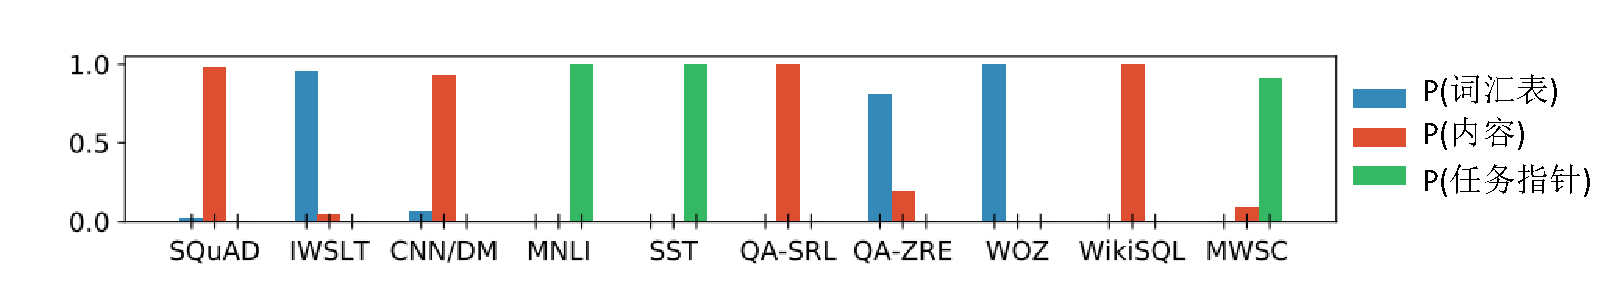
\includegraphics[width=15cm]{example/cnl2sqlselect.pdf}
  \bicaption[多任务学习网络输出来源]
    {多任务学习网络输出来源}
    {The Source of Multitasking Network Output}
  \label{fig:cnl2sqlselect}
\end{figure}

\textbf{(1) 多指针生成器与任务识别}

多任务学习网络会从三个方面进行选择:从词汇表生成词汇、任务序列上的指针以及内容序列上的指针。
尽管模型没有明确的监督信号来训练这些选择,但网络仍可以学会如何在这三个选择之间进行切换。
图\ref{fig:cnl2sqlselect}显示了本文最好的模型选择每个选项的频率是怎样的。
可以看出,对于SQuAD,QA-SRL和WikiSQL任务,模型主要是从内容信息中进行选择和复制,这正是因为这些任务中的正确结果主要攘括在内容中。
由于答案的摘要主要由内容中的单词组成,模型在CNN/DM任务中也是主要从内容中进行复制。
对于SST,MNLI和MWSC,由于任务序列中会包含需要的类别,所以模型也偏向选择任务指针。
对于IWSLT和WOZ,模型更喜欢选择从词汇表生成单词,因为中文的单词和对话的状态字段很少在对应的内容信息中。

同时,使用了TCR模板之后的所有任务之间不会使得模型产生混淆。例如:中文单词仅仅会在中文翻译成英文的过程中出现,而在情感分析任务中也从未输出过非“正面”或“负面”的情感类别。

\textbf{(2) 模型的拓展性}

多任务学习网络具有很好的拓展性,除了中文翻译为英文任务和英文生成SQL自然语言任务外对图\ref{cnl2sql:syyfx}中的其他任务都有很好的表现。
在这十个任务共同学习的模型的基础上进行其他任务的学习更加表现了模型良好的拓展性。
对于两个新的任务,英文到捷克语的翻译任务以及命名实体识别(NER)上,使用训练好的模型进行微调可以在更少的迭代次数下达到模型的收敛,达到很好的效果。
其中,英文到捷克语的翻译任务使用的是En->Cs数据集,NER任务使用的是OntoNotes 5.0数据集\cite{Hovy2006OntoNotes}。

\textbf{(3) 文本分类的零样本学习}

由于MNLI包含在是个任务中,因此模型也可以适应斯坦福自然语言推理语料库(SNLI)\cite{Bowman2015A}。
在预训练的多任务学习网络之上进行微调可以达到87%的精确匹配分数,比随机初始化再训练提升了2分,也比现有的最高水平提升了了2分\cite{Kim2018Semantic}。
更值得注意的是,在没有对SNLI进行任何微调的情况下,在原模型上预训练的多任务学习网络仍然达到了62%的精确匹配分数。
因为十个任务包含SST任务,所以它也可以在其他二元情感分类任务上表现良好。 
在亚马逊和Yelp评论数据集\cite{Kotzias2015From}上,预训练的多任务学习网络分别达到了82.1\%和80.8\%的精确匹配分数并且不需要对模型进行任何微调。
这些结果表明在多任务学习网络模型的基础上进行微调可以是的模型拓展到域外的问题上,甚至可以适应更广的文本分类问题上。

\section{本章小结}

为了进一步提高NL2SQL生成的准确性以及解决中文自然语言生成SQL查询语句的问题,本章提出了一种基于多任务学习的NL2SQL生成方法。
本方法设计了TCR模板,将中文自然语言转换为英文自然语言任务和英文自然语言转换为SQL查询语句任务进行统一。
接着,提出了由编码器和解码器构成的多任务学习网络模型。
其中,编码过程包含单独编码、对准、对偶协同注意力、压缩、自注意力和最终编码阶段;
解码过程包含结果表示、自注意力、获得中间状态、任务与内容注意力、获得任务与内容状态、多指针生成阶段。
最后,进行了多任务学习实验和优化策略实验。
实验结果表明,本文方法能够很好地完成中文自然语言生成SQL语言任务,逻辑形式准确率和数据库执行准确率达到78.7\%和86.1\%,同时还具有很好的可拓展性。
